% !TEX encoding = UTF-8
%Koma article
\documentclass[fontsize=12pt,paper=letter,twoside]{scrartcl}
\usepackage{float}
\usepackage{listings}
\usepackage{makecell}

%Standard Pre-amble
\usepackage[top=4cm,bottom=4cm,left=3cm,right=3cm,asymmetric]{geometry}
%\geometry{landscape}                % Activate for for rotated page geometry
%\usepackage[parfill]{parskip}    % Begin paragraphs with an empty line rather than an indent
\usepackage[table,xcdraw]{xcolor}
\usepackage{graphicx}

\usepackage{amsmath}
\usepackage{amssymb}
\usepackage{epstopdf}
\DeclareGraphicsRule{.tif}{png}{.png}{`convert #1 `dirname #1`/`basename #1 .tif`.png}
% Listings needs package courier
\usepackage{listings} % Needs 
\usepackage{courier}

\usepackage[framemethod=TikZ]{mdframed}
\usepackage{url}

\usepackage{sty/bsymb} %% Event-B symbols
\usepackage{sty/eventB} %% REQ and ENV
\usepackage{sty/calculation}

%Maths
\usepackage{amssymb,amsmath}
\def\Fl{\mathbb{F}}
\def\Rl{\mathbb{R}}
\def\Nl{\mathbb{N}}
\def\Bl{\mathbb{B}}
\def\St{\mathbb{S}}
\newcommand{\ovr}{\upharpoonright}
\newcommand{\var}[1]{\textit{#1}}
%Useful definitions
\newcommand{\mv}[1]{\textit{m\_#1}}
\newcommand{\cv}[1]{\textit{c\_#1}}
\newcommand{\degree}[1]{^{\circ}\mathrm{#1}}
%\newcommand{\comment}[1]{{\footnotesize \quad\texttt{--}\textrm{#1}}}
\newcommand{\im}[1]{i\texttt{-\!#1}}

\usepackage[headsepline]{scrpage2}
\pagestyle{scrheadings}
\ihead[]{\small EECS4312 Report1}
\ohead[]{\small \thepage}
\cfoot[]{}
\ofoot[]{}


%%%%PVS environment%%%%%%%%%%%%%%%%%%%
\lstnewenvironment{pvs}[1][]
    {\lstset{#1,captionpos=b,language=pvs,
    mathescape=true,
    basicstyle=\small\ttfamily,
    numbers=none,
    frame=single,
    % numberstyle=\tiny\color{gray},
    % backgroundcolor=\color{lightgray},
    firstnumber=auto
    }}
    {}
 %%%%%%%%%%%%%%%%%%%%%%%%%%%%%%%%
 
%%%%Verbatim environment%%%%%%%%%%%%%%%%%%%
\lstnewenvironment{code}[1][]
    {\lstset{#1,captionpos=b,
    mathescape=true,
    basicstyle=\small\ttfamily,
    numbers=none,
    frame=single,
    % numberstyle=\tiny\color{gray},
    % backgroundcolor=\color{lightgray},
    firstnumber=auto
    }}
    {}

% \newenvironment{boxed}[1]
%    {\begin{center}
%    #1\\[1ex]
%    \begin{tabular}{|p{0.9\textwidth}|}
%    \hline\\
%    }
%    { 
%    \\\\\hline
%    \end{tabular} 
%    \end{center}
%    }
 %%%%%%%%%%%%%%%%%%%%%%%%%%%%%%%%
 
 %Text in a box
\newenvironment{textbox}
    {\begin{center}
    \begin{tabular}{|p{0.9\textwidth}|}
    \hline\\
    }
    { 
    \\\\\hline
    \end{tabular} 
    \end{center}
    }

\usepackage{hyperref}

%Highlight \hl{}
\usepackage{soul}

\usepackage{enumitem}
\newlist{mylist}{itemize}{1}
\setlist[mylist]{label=\textbullet,leftmargin=1cm,nosep}

\usepackage{multirow}

% Reduce space between figure and caption
%\usepackage{caption}
%\captionsetup[table]{font=small,skip=0pt}     %% Adjust here
%or equivalently 
\usepackage[font=small,skip=4pt]{caption}
%Useful definitions
%\newcommand{\mv}[1]{\textit{m\_#1}}
%\newcommand{\cv}[1]{\textit{c\_#1}}
%\newcommand{\degree}[1]{^{\circ}\mathrm{#1}}
%\newcommand{\comment}[1]{{\footnotesize \quad\texttt{--}\textrm{#1}}}


%For Code Stylings
\usepackage{listings}
\usepackage{color}

\definecolor{dkgreen}{rgb}{0,0.6,0}
\definecolor{gray}{rgb}{0.5,0.5,0.5}
\definecolor{mauve}{rgb}{0.58,0,0.82}

\lstset{frame=tb,
  language=Java,
  aboveskip=3mm,
  belowskip=3mm,
  showstringspaces=false,
  columns=flexible,
  basicstyle={\small\ttfamily},
  numbers=none,
  numberstyle=\tiny\color{gray},
  keywordstyle=\color{blue},
  commentstyle=\color{dkgreen},
  stringstyle=\color{mauve},
  breaklines=true,
  breakatwhitespace=true,
  tabsize=3
}

% Set the header
\ihead[]{\small EECS4313 Assignment-3}


%%%%%%%%%%%%Enter your names here%%%%%%%%
\author{Student Name | Student Number | EECS Account
\and \textbf{Edward Vaisman | 212849857 | eddyv}
\and \textbf{Robin Bandzar | 212200531 | cse23028}
\and \textbf{Kirusanth Thiruchelvam | 212918298 | kirusant}
\and \textbf{Sadman Sakib Hasan | 212497509 | cse23152}
}
%%%%%%%%%%%%%%%%%%%%%%%%%%%%%%%%

\date{\today} % Display a given date or no date

\begin{document}
\title{EECS 4313 Assignment 3 \\Data Flow Testing, Slice-Based Testing and Mutation Testing}
\maketitle

\newpage

%%%%%%%%%%%%%%%%%%%%%%%%%%%%%%%
\tableofcontents


\newpage


\section{BORG Calendar}

\subsection{Data Flow Testing}

\subsubsection{Chosen Method}

\begin{itemize}
\item \textbf{Class}: \emph{net.sf.borg.common.DateUtil.java}
\item \textbf{Method}: \emph{minuteString(int mins)}
\item \textbf{Method Description}:
This method generate a human reable string for a particular number of minutes. It returns the string in terms of hours or minutes or both hours and mintues.
\begin{itemize}
\item \textbf{mins} - The first argument is of type integer.
\end{itemize}
\end{itemize}

\noindent Following is the code snippet of the \emph{minuteString} method:
\begin{code}
	public static String minuteString(int mins) {
		
		int hours = mins / 60;
		int minsPast = mins % 60;
		
		String minutesString;
		String hoursString;
		
		if (hours > 1) {
			hoursString = hours + " " + Resource.getResourceString("Hours");
		} else if (hours > 0) {
			hoursString = hours + " " + Resource.getResourceString("Hour");
		} else {
			hoursString = "";
		}

		if (minsPast > 1) {
			minutesString = minsPast + " " + Resource.getResourceString("Minutes");
		} else if (minsPast > 0) {
			minutesString = minsPast + " " + Resource.getResourceString("Minute");
		} else if (hours >= 1) {
			minutesString = "";
		} else {
			minutesString = minsPast + " " + Resource.getResourceString("Minutes");
		}

		// space between hours and minutes
		if (!hoursString.equals("") && !minutesString.equals(""))
			minutesString = " " + minutesString;

		return hoursString + minutesString;
	}
\end{code}

\subsubsection{Variable set}

Following are the list of variables used in the \emph{minuteString} method along with their types:

\begin{table}[h]
\centering
\begin{tabular}{|c | c | c |}
	\cline{1-3}
	\textbf{Variable Name} & \textbf{Data Type} & \textbf{Is Primitive?}\\ \hline
	mins & int & Yes \\ \hline
	hours & int & Yes \\ \hline
	minsPast & int & Yes \\ \hline
	minutesString & String & No \\ \hline
	hoursString & String & No \\ \hline
\end{tabular}
\caption {List of variables for the minuteString method}
\label{tbl:list_variables}
\end{table}

\noindent \textbf{Note}: The last two variables, \emph{minutesString} and \emph{hoursString}, are \textbf{NOT} primitive types, and will \textbf{NOT} be used to perform the data flow analysis as specified by the instructor.

\subsubsection{Program Segmentation}

The following table \ref{tbl:program_segmentation} contains the \emph{minuteString} method broken down into segments:

\begin{table}[h]
\centering
\begin{tabular}{|c | c |}
	\cline{1-2}
	public static string minuteString(int mins) & A \\ \hline
	int hours = mins / 60; & \\ 
	int minsPast = mins \% 60; & B \\ \hline
	String minutesString; & \\ 
	String hoursString; & C \\ \hline
	if (hours $>$ 1) \{ & D \\ \hline
	hoursString = hours + " " + Resource.getResourceString("Hours"); & E \\ \hline
	\} else if (hours $>$ 0) \{ & F \\ \hline
	hoursString = hours + " " + Resource.getResourceString("Hour"); & G \\ \hline
	\} else \{ hoursString = ""; \} & H \\ \hline
	if (minsPast $>$ 1) \{ & I \\ \hline
	minutesString = minsPast + " " + Resource.getResourceString("Minutes"); & J \\ \hline
	\} else if (minsPast $>$ 0) \{ & K \\ \hline
	minutesString = minsPast + " " + Resource.getResourceString("Minute"); & L \\ \hline
	\} else if (hours $>=$ 1) \{ & M \\ \hline
	minutesString = ""; & N \\ \hline
	\} else \{ & \\ 
	minutesString = minsPast + " " + Resource.getResourceString("Minutes"); & O \\
	\} & \\ \hline
	if (!hoursString.equals("") \&\& !minutesString.equals("")) & P \\ \hline
	minutesString = " " + minutesString; & Q \\ \hline
	return hoursString + minutesString; & R \\ \hline
\end{tabular}
\caption {Program Segmentation for the minuteString method}
\label{tbl:program_segmentation}
\end{table}

\newpage
\subsubsection{Program graph}
The following diagram \ref{fig:cfg} represents the control flow graph for the \emph{minuteString} method:

\begin{figure}[!htb]
\begin{center}
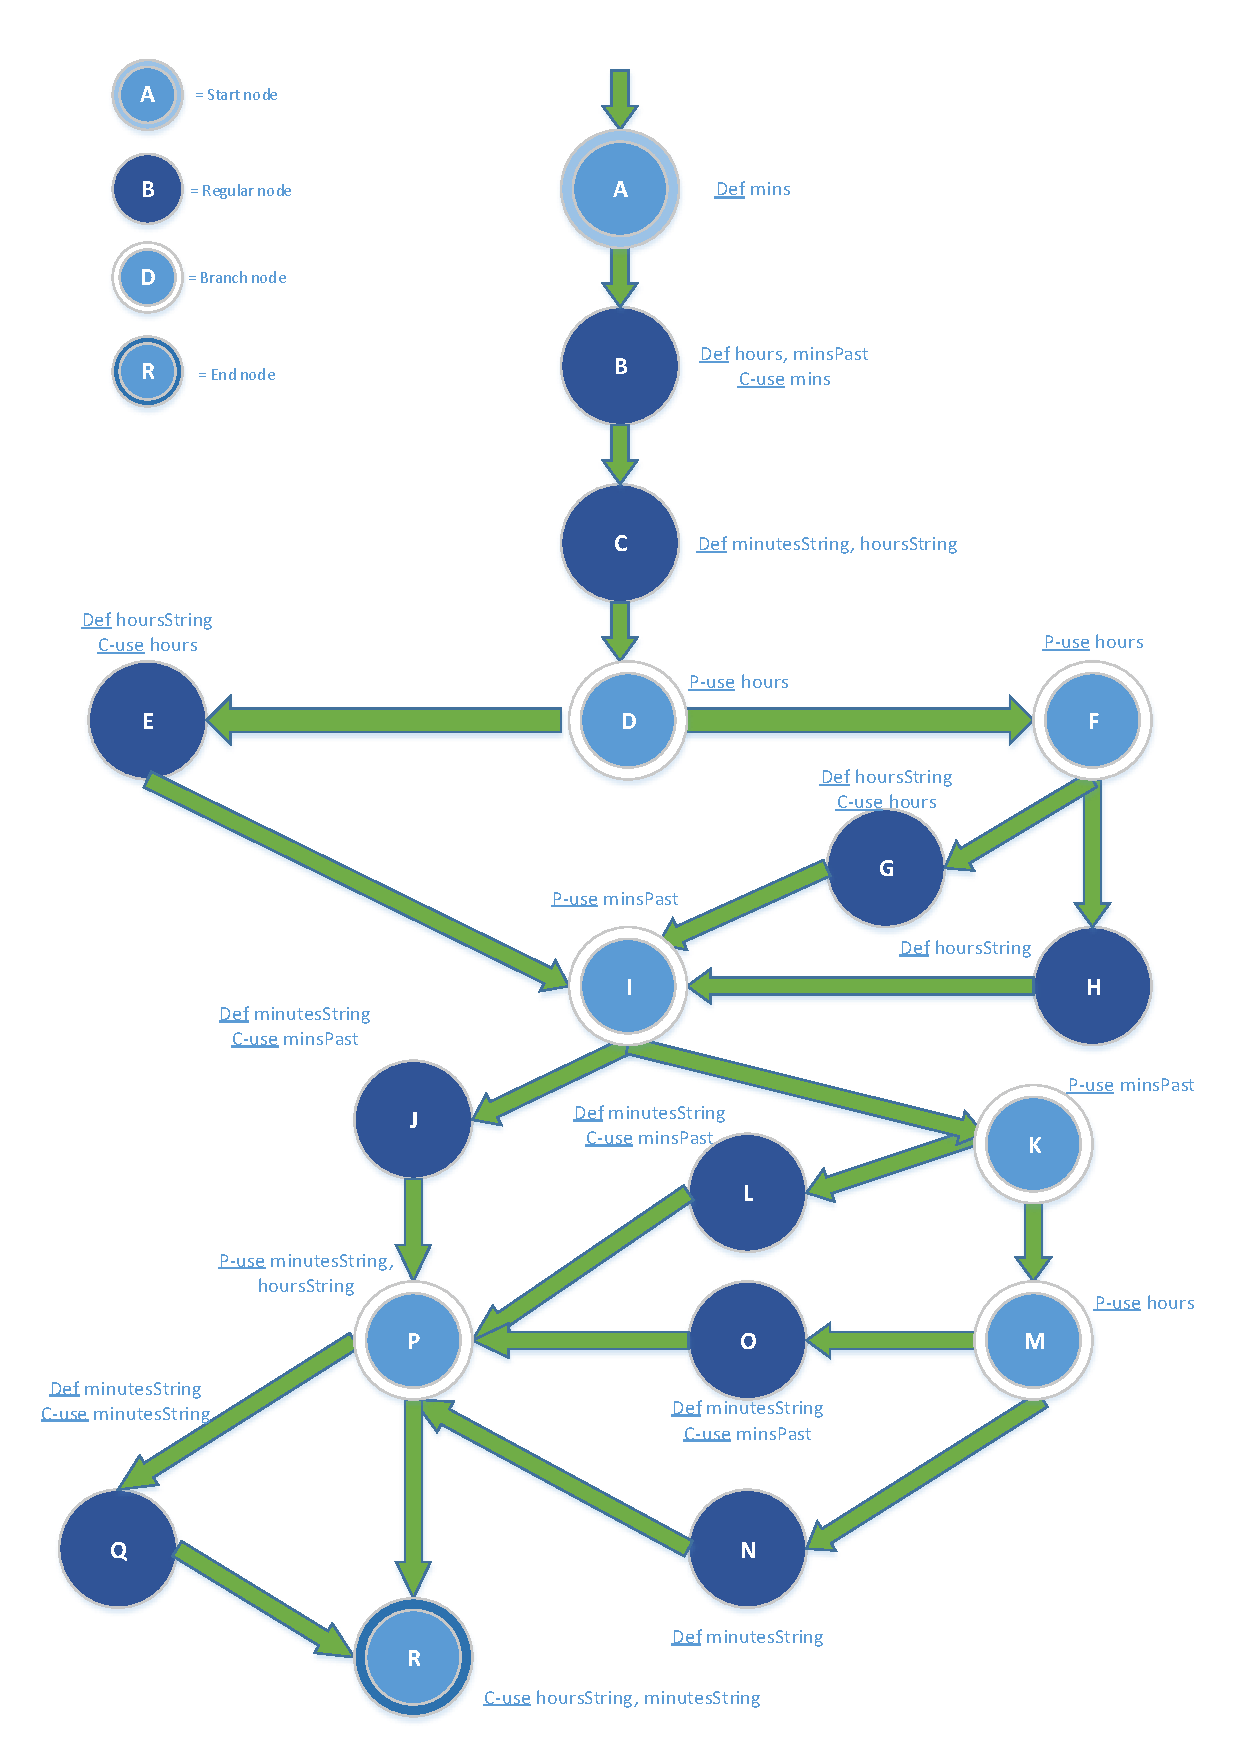
\includegraphics[width=.99\textwidth]{images/dft/cfg.pdf}
\end{center}
\caption{Control Flow Graph for the minuteString method}
\label{fig:cfg}
\end{figure}

\clearpage
\newpage
\subsubsection{Data Flow Analysis}

\begin{enumerate}
\item \textbf{du-paths for \emph{mins}}
\begin{itemize}
\item \textbf{All-Defs}: \emph{AB}
\item \textbf{All-C-Uses/Some-P-Uses}: \emph{AB}
\item \textbf{All-P-Uses/Some-C-Uses}: \emph{AB}
\item \textbf{All-Uses}: \emph{AB}
\end{itemize}

\item \textbf{du-paths for \emph{hours}}
\begin{itemize}
\item \textbf{All-Defs}: \emph{BCD}
\item \textbf{All-C-Uses/Some-P-Uses}: \emph{BCDE, BCDFG}
\item \textbf{All-P-Uses/Some-C-Uses}: \emph{BCD, BCDF, BCDEIKM, BCDFGIKM, BCDFHIKM}
\item \textbf{All-Uses}: \emph{BCD, BCDE, BCDF, BCDEIKM, BCDFG, BCDFGIKM, BCDFHIKM}
\end{itemize}

\item \textbf{du-paths for \emph{minsPast}}
\begin{itemize}
\item \textbf{All-Defs}: \emph{BCDEI}
\item \textbf{All-C-Uses/Some-P-Uses}: \emph{BCDEIJ, BCDFGIJ, BCDFHIJ, BCDEIKL, BCDFGIKL, BCDFHIKL, BCDEIKMO, BCDFGIKMO, BCDFHIKMO}
\item \textbf{All-P-Uses/Some-C-Uses}: \emph{BCDEI, BCDFGI, BCDFHI, BCDEIK, BCDFGIK, BCDFHIK}
\item \textbf{All-Uses}: \emph{BCDEI, BCDEIJ, BCDFGIJ, BCDFHIJ, BCDEIKL, BCDFGIKL, BCDFHIKL, BCDEIKMO, BCDFGIKMO, BCDFHIKMO, BCDFGI, BCDFHI, BCDEIK, BCDFGIK, BCDFHIK}
\end{itemize}

\end{enumerate}


\subsubsection{Coverage Metrics}

Following are the existing test cases from Assignment-2 and their coverage metrics using the data flow analysis for the \emph{minuteString} method:

\begin{enumerate}

\item \textbf{Test Case 1}:
\begin{itemize}
\item \textbf{Input}: mins = 60
\item \textbf{Path}: \emph{ABCDEGIKMNPR}
\item \textbf{Coverage}: 100*(12/18) = 66.67\%
\end{itemize}

\item \textbf{Test Case 2}:
\begin{itemize}
\item \textbf{Input}: mins = 61
\item \textbf{Path}: \emph{ABCDFGIKLPQR}
\item \textbf{Coverage}: 100*(14/18) = 77.78\%
\end{itemize}

\item \textbf{Test Case 3}:
\begin{itemize}
\item \textbf{Input}: mins = 75
\item \textbf{Path}: \emph{ABCDFGIJPQR}
\item \textbf{Coverage}: 100*(15/18) = 83.33\%
\end{itemize}

\item \textbf{Test Case 4}:
\begin{itemize}
\item \textbf{Input}: mins = 180
\item \textbf{Path}: \emph{ABCDEIKMNPR}
\item \textbf{Coverage}: 100*(16/18) = 88.88\%
\end{itemize}

\item \textbf{Test Case 5}:
\begin{itemize}
\item \textbf{Input}: mins = 121
\item \textbf{Path}: \emph{ABCDEIKLPQR}
\item \textbf{Coverage}: 100*(16/18) = 88.88\%
\end{itemize}

\item \textbf{Test Case 6}:
\begin{itemize}
\item \textbf{Input}: mins = 145
\item \textbf{Path}: \emph{ABCDEIJPQR}
\item \textbf{Coverage}: 100*(16/18) = 88.88\%
\end{itemize}

\item \textbf{Test Case 7}:
\begin{itemize}
\item \textbf{Input}: mins = 0
\item \textbf{Path}: \emph{ABCDFHIOPR}
\item \textbf{Coverage}: 100*(18/18) = 100.0\%
\end{itemize}

\end{enumerate}

\noindent \textbf{Rationale}: The testing technique used for testing this method is \emph{Equivalence Class Testing}. It is a suitable technique for this method since the argument is an integer which is an independent variable and the input range can be partitioned assuring disjointness and non-redundancy between each partition set. We have chosen the partition integer range based on usages of minute, minutes, hour, and hours. In order to partition the integer argument into hours and minutes, we divide the minutes by 60 to get the range of hours and the remainder (minutes \% 60) to get the range of the minutes. By covering all the cases, where the given input returns a concatenation of hours and minutes string, we were able to reach a 100\% coverage for this method.

\newpage
\begin{itemize}
\item The data flow analysis you performed and the calculation of the coverage metrics. You must
show which test cases are responsible for which dc-paths.
\item A description of the test cases you added to improve coverage. If your coverage was already high,
discuss how your testing was able to achieve this.
\item The slices that you identified and the percentage of slices that your testing covers. You must
show which test cases are responsible for which slices.
\item A description of the test cases you added to improve slice coverage. If your coverage was
already high, discuss how your testing was able to achieve this.
\item Evaluate the effectiveness of your test cases using mutation testing. Discuss and address any
issues if you have found in your written report.
\item Attaching bug reports if bugs are discovered using your testing methods. You should use the
same bug report format as in Assignment 1. Do not file these bug reports to the project’s bug
report system.
\item An appendix with the specification of the methods you are testing
\end{itemize}

\section{JPetStore}

\begin{itemize}
\item The test scenarios that you have created;
\item The request rates and the duration of the load tests;
\item The analysis of your load tests and the description of any problems that you have found (if there
are any).
\end{itemize}

\end{document}
